\documentclass{article}

\title{Part 3: Team of Teams\\Chapters 7 to 10}
\author{Vladimir Feinberg}

% latex math commands
% Vladimir Feinberg
% \vx notation for vectors from Goodfellow
% https://github.com/goodfeli/dlbook_exercises

% alphabet templates
% abcdefghijklmnopqrstuvwxyz
% ABCDEFGHIJKLMNOPQRSTUVWXYZ

% fonts, math, and layout commands
\usepackage{fullpage}


\usepackage{setspace} % for \onehalfspacing and \singlespacing macros
\onehalfspacing 

\usepackage{etoolbox}
\AtBeginEnvironment{quote}{\singlespacing\small}

\usepackage{bbm}
\usepackage{enumerate}
\usepackage{amsmath}
\usepackage{amsthm}
\usepackage{amssymb}
\usepackage{amsfonts}
\usepackage{mathrsfs}
\usepackage{mathtools}
\usepackage[all]{xy}

% include graphics with \includegraphics
\usepackage{graphicx}
\usepackage{caption}

% \nicefrac{x}{y} gives a diagonal fraction bar x/y
\usepackage{nicefrac}

% \nurl{<url>}{link name} renders a blue underlined link
\usepackage[hidelinks]{hyperref}
\usepackage{xcolor}
\usepackage{url}
\newcommand{\nurl}[2]{\href{ #1 }{\color{blue}\underline{#2}}}

% brackets, norms, cardinalities
\newcommand{\pa}[1]{ \left({#1}\right) }
\newcommand{\ha}[1]{ \left[{#1}\right] }
\newcommand{\ca}[1]{ \left\{{#1}\right\} }
\newcommand{\inner}[1]{\left\langle #1 \right\rangle}
\newcommand{\innercpy}[1]{\inner{ #1, #1 }}
\newcommand{\norm}[1]{\left\lVert #1 \right\rVert}
\newcommand{\card}[1]{\left\lvert{#1}\right\rvert}
\newcommand{\abs}[1]{\card{#1}}

% math vectors
\newcommand{\va}{\textbf{a}}
\newcommand{\vb}{\textbf{b}}
\newcommand{\vc}{\textbf{c}}
\newcommand{\vd}{\textbf{d}}
\newcommand{\ve}{\textbf{e}}
\newcommand{\vf}{\textbf{f}}
\newcommand{\vg}{\textbf{g}}
\newcommand{\vh}{\textbf{h}}
\newcommand{\vi}{\textbf{i}}
\newcommand{\vj}{\textbf{j}}
\newcommand{\vk}{\textbf{k}}
\newcommand{\vl}{\textbf{l}}
\newcommand{\vm}{\textbf{m}}
\newcommand{\vn}{\textbf{n}}
\newcommand{\vo}{\textbf{o}}
\newcommand{\vp}{\textbf{p}}
\newcommand{\vq}{\textbf{q}}
\newcommand{\vr}{\textbf{r}}
\newcommand{\vs}{\textbf{s}}
\newcommand{\vt}{\textbf{t}}
\newcommand{\vu}{\textbf{u}}
\newcommand{\vv}{\textbf{v}}
\newcommand{\vw}{\textbf{w}}
\newcommand{\vx}{\textbf{x}}
\newcommand{\vy}{\textbf{y}}
\newcommand{\vz}{\textbf{z}}
\newcommand{\vzero}{\textbf{0}}
\newcommand{\vone}{\textbf{1}} 
\newcommand{\valpha}{{\boldsymbol\alpha}}
\newcommand{\vepsilon}{{\boldsymbol\epsilon}}
\newcommand{\veta}{{\boldsymbol\eta}}
\newcommand{\vsigma}{ {\boldsymbol\sigma}}
\newcommand{\vtheta}{ {\boldsymbol\theta}}
\newcommand{\vdelta}{ {\boldsymbol\delta}}
\newcommand{\vlambda}{ {\boldsymbol\lambda}}
\newcommand{\vmu}{ {\boldsymbol\mu}}
\newcommand{\vvartheta}{ {\boldsymbol\vartheta}}
\newcommand{\vbeta}{ {\boldsymbol\beta}}
\newcommand{\vphi}{ {\boldsymbol\phi}}


% math function arrows, misc binary math ops
\newcommand{\bij}{\leftrightarrow}
\newcommand{\inj}{\rightarrowtail}
\newcommand{\sur}{\twoheadedrightarrow}
\newcommand{\eqd}{\mathrel{\overset{\Delta}{=}}}

% common math sets
\newcommand{\Z}{\mathbb{Z}}
\newcommand{\R}{\mathbb{R}}
\newcommand{\C}{\mathbb{C}}
\newcommand{\N}{\mathbb{N}}
\newcommand{\Q}{\mathbb{Q}}
\newcommand{\F}{\mathbb{F}}
\newcommand{\T}{\mathbb{T}}

% limits
\def\sumn{\sum_{n=0}^\infty}
\def\limn{\lim_{n\rightarrow\infty}}
\def\prodn{\prod_{n=0}^\infty}

% mathcal
\newcommand{\mcA}{\mathcal{A}}
\newcommand{\mcB}{\mathcal{B}}
\newcommand{\mcC}{\mathcal{C}}
\newcommand{\mcD}{\mathcal{D}}
\newcommand{\mcE}{\mathcal{E}}
\newcommand{\mcF}{\mathcal{F}}
\newcommand{\mcG}{\mathcal{G}}
\newcommand{\mcH}{\mathcal{H}}
\newcommand{\mcI}{\mathcal{I}}
\newcommand{\mcJ}{\mathcal{J}}
\newcommand{\mcK}{\mathcal{K}}
\newcommand{\mcL}{\mathcal{L}}
\newcommand{\mcM}{\mathcal{M}}
\newcommand{\mcN}{\mathcal{N}}
\newcommand{\mcO}{\mathcal{O}}
\newcommand{\mcP}{\mathcal{P}}
\newcommand{\mcQ}{\mathcal{Q}}
\newcommand{\mcR}{\mathcal{R}}
\newcommand{\mcS}{\mathcal{S}}
\newcommand{\mcT}{\mathcal{T}}
\newcommand{\mcU}{\mathcal{U}}
\newcommand{\mcV}{\mathcal{V}}
\newcommand{\mcW}{\mathcal{W}}
\newcommand{\mcX}{\mathcal{X}}
\newcommand{\mcY}{\mathcal{Y}}
\newcommand{\mcZ}{\mathcal{Z}}

% measure theory, distributions
\newcommand{\indicator}{\mathbbm{1}}
\DeclareMathOperator{\Laplace}{Laplace}
\DeclareMathOperator{\soft}{soft}
\DeclareMathOperator{\hard}{hard}
\DeclareMathOperator{\clo}{clo}
\DeclareMathOperator{\Poisson}{Poisson}
\DeclareMathOperator{\Exponential}{Exponential}
\DeclareMathOperator{\Multinomial}{Multinomial}
\DeclareMathOperator{\Bernoulli}{Bernoulli}
\DeclareMathOperator{\Categorical}{Categorical}
\DeclareMathOperator{\Uniform}{Uniform}
\DeclareMathOperator{\Binomial}{Binomial}
\DeclareMathOperator{\Hypergeometric}{Hypergeometric}
\DeclareMathOperator{\GammaDist}{Gamma}
\DeclareMathOperator{\NegativeBinomial}{NegativeBinomial}
\DeclareMathOperator\mathProb{\mathbb{P}}
\DeclareMathOperator\sub{sub}
\renewcommand{\d}[1]{\mathop{\mathrm{d} #1 }}
\DeclarePairedDelimiterX{\infdivx}[2]{(}{)}{ #1\;\delimsize\|\;#2 }
\newcommand{\dkl}[2]{\mathop{D_\text{KL}}\infdivx{#1}{#2}}
\newcommand{\sg}{\mathop{\mathrm{SG}}}
\newcommand{\se}{\mathop{\mathrm{SE}}}

% distributions
\makeatletter
\newcommand{\distas}[1]{\mathbin{\overset{#1}{\kern\z@\sim}}}%
\makeatother
\newcommand{\disteq}{\overset{d}{=}}
\newcommand{\distiid}{\distas{\text{iid}}}
\newcommand\independent{\protect\mathpalette{\protect\independenT}{\perp}}
\def\independenT#1#2{\mathrel{\rlap{$#1#2$}\mkern2mu{#1#2}}}
\newcommand{\convdist}{\mathbin{\overset{\text{d}}{\longrightarrow}}}
\newcommand{\convas}{\mathbin{\overset{\text{as}}{\longrightarrow}}}
\newcommand{\convpb}{\mathbin{\overset{\text{pb}}{\longrightarrow}}}

\renewcommand{\P}{\mathProb} % need to overwrite stupid paragraph symbol
\DeclareMathOperator\mathExp{\mathbb{E}}
\DeclareMathOperator*\mathExpUnder{\mathbb{E}}
\newcommand{\E}{\mathExp}

\newcommand{\sa}{{$\sigma$-algebra}}
\newcommand{\OR}{{\overline{\R}}}
\newcommand{\OX}{{\overline{X}}}
\DeclareMathOperator{\power}{{\mathcal{P}}}
\DeclareMathOperator{\var}{var}
\DeclareMathOperator{\cov}{cov}

% \set{from set}{condition} with set-builder notation
% conditional expectation is analogous
\newcommand{\set}[2]{ \left\{ #1 \,\middle|\, #2 \right\} }
\newcommand{\CE}[2]{ \mathExp\left[ #1 \,\middle|\, #2 \right] }
\newcommand{\CP}[2]{ \mathProb\left\{ #1 \,\middle|\, #2 \right\} }

% linear-algebra related
\newcommand{\rip}{\operatorname{RIP}}
\DeclareMathOperator{\svd}{svd}
\newcommand{\frob}[1]{\norm{#1}_{\mathrm{F}}}
\newcommand{\mat}[1]{\begin{pmatrix} #1 \end{pmatrix}}
\newcommand{\detmat}[1]{\begin{vmatrix} #1 \end{vmatrix}}
\DeclareMathOperator{\spanb}{span}
\DeclareMathOperator{\conv}{conv} % convex hull
\DeclareMathOperator{\cone}{cone}
\DeclareMathOperator{\vectorize}{vec}
\DeclareMathOperator{\matricize}{mat}
\DeclareMathOperator{\adj}{adj}
\DeclareMathOperator{\diag}{diag}
\DeclareMathOperator{\tr}{tr}
\DeclareMathOperator{\rank}{rank}
\DeclareMathOperator*{\argmin}{argmin}
\DeclareMathOperator*{\argmax}{argmax}
\DeclareMathOperator*{\proj}{proj}

% complex analysis
\DeclareMathOperator{\MyRe}{Re}
\DeclareMathOperator{\MyIm}{Im}
\DeclareMathOperator{\image}{image}
\DeclareMathOperator{\supp}{supp}

% typical numerical operators
\DeclareMathOperator{\sgn}{sgn}

% graphs
\DeclareMathOperator{\diam}{diam}

% constants
\renewcommand{\d}[1]{\mathop{\mathrm{d} #1 }}
\newcommand{\e}{\mathrm{e}}
\renewcommand{\i}{\imath}

% \bigtimes: large indexed cross product
\makeatletter
\DeclareFontFamily{U}  {MnSymbolF}{}
\DeclareSymbolFont{symbolsMN}{U}{MnSymbolF}{m}{n}
\SetSymbolFont{symbolsMN}{bold}{U}{MnSymbolF}{b}{n}
\DeclareFontShape{U}{MnSymbolF}{m}{n}{
    <-6>  MnSymbolF5
   <6-7>  MnSymbolF6
   <7-8>  MnSymbolF7
   <8-9>  MnSymbolF8
   <9-10> MnSymbolF9
  <10-12> MnSymbolF10
  <12->   MnSymbolF12}{}
\DeclareFontShape{U}{MnSymbolF}{b}{n}{
    <-6>  MnSymbolF-Bold5
   <6-7>  MnSymbolF-Bold6
   <7-8>  MnSymbolF-Bold7
   <8-9>  MnSymbolF-Bold8
   <9-10> MnSymbolF-Bold9
  <10-12> MnSymbolF-Bold10
  <12->   MnSymbolF-Bold12}{}
\DeclareMathSymbol{\tbigtimes}{\mathop}{symbolsMN}{2}
\newcommand*{\bigtimes}{%
  \DOTSB
  \tbigtimes
  \slimits@ 
}
\makeatother

% category theory arguments
% See https://tex.stackexchange.com/questions/356873
\newcommand{\catfst}{{-}}
\newcommand{\catsnd}{{=}}
\newcommand{\cattrd}{{\equiv}}
\DeclareMathOperator{\Id}{Id}
\newcommand{\opcat}[1]{{#1}^{\text{op}}}
\DeclareMathOperator{\Hom}{hom}
\DeclareMathOperator{\Ob}{ob}
\DeclareMathOperator{\El}{el}
\DeclareMathOperator{\colim}{colim}
\DeclareMathOperator{\Sym}{Sym}
% restriction of a function to a domain
\newcommand\restr[2]{{% we make the whole thing an ordinary symbol
  \left.\kern-\nulldelimiterspace % automatically resize the bar with \right
  #1 % the function
  \vphantom{\big|} % pretend it's a little taller at normal size
  \right|_{#2} % this is the delimiter
  }}
\usepackage[all]{xy}


\begin{document}

\maketitle

Notes on Chapters 7 to 10 of Andy Grove's \textit{High Output Management} \cite{highoutput}.

Note that the sections are structured according to topics, not the chapters themselves.

\section{The Centralization-Decentralization Dichotomy}

Modern organizations need to carefully walk the centralization-decentralization tradeoff line.
Centralization permits more consistent quality and take advantage of economies at scale, but at the same time decentralization allows for local optimization (profits, increases in quality, reduction in costs by taking advantage of local offerings).

Conglomerates used to own entire verticals globally, but now there is increasing national support and competitors on a global business scene.
Uber lost to a Chinese mobile app for transportation because of national support and localization advantages.

Centralization/decentralization decisions need to be made in a way that effectively organizes a team of teams.

\begin{itemize}
\item An instance where centralization is a poor choice would be in setting a payscale for a franchise. Local branch managers would likely have a better sense of what the standards for a particular region (including local factors like cost of living) would be. Analogously, local managers likely have the best context to make decisions about hiring or firing employees.
\item However, multiple business units in a single-objective software company would likely conflict. This occurs in practice, resulting in sales teams within the same company fighting over the same customers. This confuses brand messaging and needlessly wastes effort when the whole company has already captured an entire account.
\end{itemize}


\section{Partitioning an Organization}

Organizations can be partitioned along two different dimensions.

\textbf{Mission-oriented} partitions, or \textbf{business units}, partition along industry verticals, with the unit taking care of all of its needs end to end for a business product (e.g., splitting into a northwest region, southwest region, etc.). These units operate individually, fulfilling their own mission

\textbf{Functional} partitions, or \textbf{functional units}, divide by separate functionalities. These are interdependent to achieve end-to-end business goals, and instead specialize on a particular horizontal in terms of what they can do.

Hybrid organizations are split along both types of units (possibly at different levels, too). This decision should be made in a way that maximizes responsiveness and managerial leverage (both can be improved by making a certain set of functional/business unit splits---the decision is context-dependent, mostly on the interaction pattern between horizontals).

When would one create a functional unit? When there are large economies of scale and deep verticals for their contractors and vendors, it makes sense to isolate that as a single functional component which has mastery over a difficult component to have high-leverage value add for a fixed amount of company resources.

When would one create a business unit? When transaction, communication, or transportation costs are large for the interaction of multiple broken down functional or business units necessary to represent the end-to-end functionality of a single business unit.

There is a \textit{fundamental tradeoff} (which makes this a useful leverage when designing an organization), which is that:
\begin{itemize}
\item Functional units need to inter- and intra-communicate well, which is costly.
\item Business units need to solve problems across their entire vertical, which is costly.
\end{itemize}

For example, Intel might extract manufacturing due to the many vendor requirements for building chips. Similarly, sales requires a shared pool of business connections (Fig.~\ref{fig:partitioning}).

\begin{figure}[h]
  \centering
  \includegraphics[height=10cm]{partitioning.pdf}
  \caption{\label{fig:partitioning} }
\end{figure}

  Facebook has VR and AR in its own building b/c it's a specialized vertical (business unit), but Infrastructure teams are spread throughout all the buildings b/c they interleave with a lot of product functionality (functional unit).

\textit{Grove's law}: eventually all large organizations hybridize.\footnote{This doesn't really say that much to me, just that the optimization is nontrivial and requires a mix of both.}

\section{Dual reporting}

Any multi-faceted, complicated organization is a system with many moving parts, each of which has a component prone to independent failure. As such, failures (or delays in general) in the system as a whole can increase with a rate exponential in the number of subcomponents.

For example, should plant security report to the local plant manager or the security manager (who is at corporate headquarters)? Need to give information to both and fulfill requests from both, so report to both. This is \textbf{dual reporting}.

What to do if a component that someone's responsible for has no corresponding manager that would own the supervision for that component's quality. For instance, plant managers might have a general manager responsible for their entire region's overall production, but there's no one to report to for technical oversight. In these cases, we can emulate a senior technical manager by combining a group of individual technical managers who are responsible for themselves. This is \textbf{group of peers} dual reporting (Fig.~\ref{fig:peers}).

\begin{figure}[h]
  \centering
  \includegraphics[height=6cm]{peers.pdf}
  \caption{\label{fig:peers} }
\end{figure}

This scenario comes up in software during, e.g., design review, in absence of a tech lead. Note that dual reporting can be performed across functional or business units.

One related but distinct concept is that of the \textbf{multi-plane organization}. Whereas dual reporting is about overlapping safeguards on a single component, multi-plane organizations assign an individual to several disjoint responsibilities. This is distinct from dual reporting because you’re reporting regarding disjoint responsibilities. Supervision does not overlap. Roles are managed, not people.

\section{Modes of Control}

There are three operational modes of control.

\begin{enumerate}
\item \textbf{Free market forces}. These are only applicable when there's a concrete value that can be established. In commodity marketplaces, this means that there is a dollar value determined for the commodity in context. In the workplace, these situations may be difficult to find, but occur in situations where vendors exchange services specified at a detailed level, e.g., software contractors for creating websites. Alternatively, concretely defined requirements for technical progression at Facebook have metrics attached (with complimentary indicators for quality). They put a number on what it takes to move up the ladder.
\item \textbf{Contractual obligations}. Long-term obligations involving coordination with a group of people require contracts (e.g., labor). For instance, the power company gets a license to access a resource by the government, effectively becoming a sponsored monopoly, but then it has to play on the same team by providing electricity at non-monopolistic prices. Alternatively, employment contracts for most salaried work specify vague duties that require adherence to a general team objective.
\item \textbf{Cultural values}. These are shared set of values, objectives, and methods. These are powerful tools, but they can be difficult to establish. They can only really be articulated and set by example and strict adherence. One concrete way of describing what corporate values really are,\footnote{This is in opposition to the common misinterpretation that quirks like workisng on doors or not wearing shoes or playing ping pong determine culture. At best, they are zealous expressions of a latent culture. The following interpretation of what company culture ``really is'' was first mentioned to me by Ali Ghodsi.} how do you approach tradeoffs as a company in a consistent way? At Facebook, do you harvest information about users in order to improve their UX, and if so where does it stop? At personally identifiable information being available to non-support engineers.
\end{enumerate}

Choosing the right mode of control depends on the situational context. Andy Grove proposes a composite index termed the \textbf{CUA factor} which is a combination of complexity, uncertainty, and ambiguity. Depending on the personal motivation that is influencing an individual in the given scenario, and the CUA factor, an appropriate mode of control can be selected (Fig.~\ref{fig:control}).

\begin{figure}[h]
  \centering
  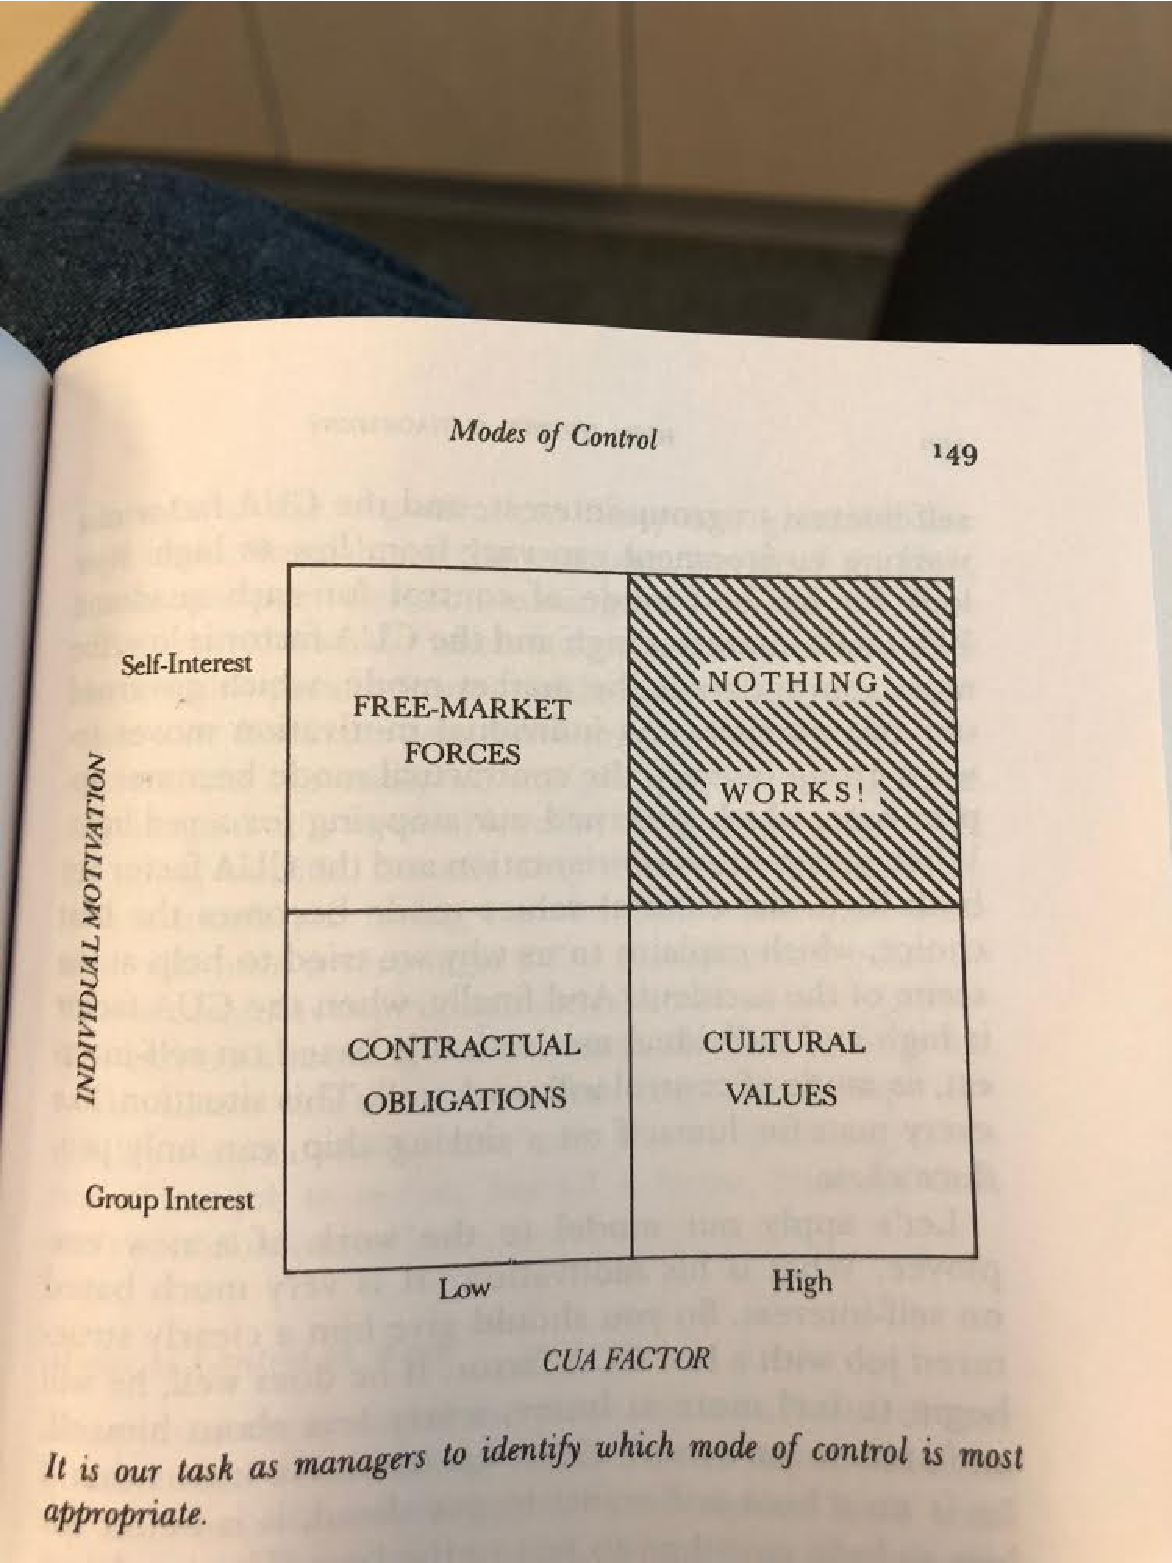
\includegraphics[height=7cm]{control.pdf}
  \caption{\label{fig:control} }
\end{figure}

High CUA and self-interest based motivation is chaotic by definition, since CUA means everyone has random objectives, and there’s no unifying aim (due to self interest).

This has an \textit{essential} implication, which is that in highly uncertain situations, progress can only be created with groups and strong culture, which is why startups require focus on culture.

\bibliography{biblio}{}
\bibliographystyle{unsrt}

\end{document}